
In this analysis, ANSYS conducts an electro-thermal simulation using the element LINK68. LINK68 is a uniaxial 1D element which can be used in a 3D space. It has the ability to conduct heat and electrical current along its nodes with an internal heat source corresponding to the Joule effect. Similarly to the element LINK33, it is used for steady-state and transient numerical problems~\cite{ansys_element_manual}. In preceding simulations, the Joule effect was implemented by introducing a power source over the entire strand domain as a function of resistivity (being a function of temperature). The usage of LINK68 allows for omitting this step since the solver computes the heat source by an internal routine based on material property state. The element requires material property for electrical resistivity of the composite strand.

In order to obtain the same solver settings as in case of the analysis performed in Section \ref{subsection:quench_velocity_benchmarking_no_insulation_heat_balance}, the 1D strand domain was grounded and constant value of current was applied, as shown in Fig. \ref{fig: q_vel_benchmarking_electrical_settings}.

\begin{figure}[H]
\centering
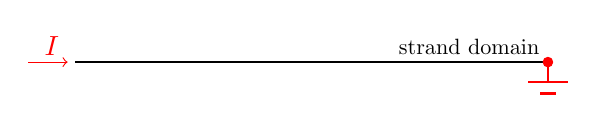
\begin{tikzpicture}[scale = 1]
\draw[thick, black] (-3,0) -- (3,0);
\filldraw[red] (3,0) circle (0.06);
\draw[thick, red] (3,0) -- (3,-0.25);
\draw[thick, red] (2.75,-0.25) -- (3.25,-0.25);
\draw[thick, red] (2.9,-0.4) -- (3.1,-0.4);
\draw[thin, red, ->] (-3.6,0) -- (-3.1,0);
\node[scale=0.8] at (2,0.2) {strand domain};
\node[scale=1.0, red] at (-3.3,0.2) {$I$};
\end{tikzpicture}
\caption{Electric boundary conditions.}
\label{fig: q_vel_benchmarking_electrical_settings}
\end{figure}

Two time step ranges were chosen: $t=\{[10, 100], [100, 1000]\}~\upmu \text{s}$. The study over a 1 metre-long domain was conducted with a varying number of nodes, $n=\{30, 50, 100, 500, 1000\}$. The geometric assumptions as well as initial conditions were the same as in Section \ref{subsection: 1D_quench_propagation_no_insulation} without a heat source. The additional parameters related to the co-simulation are shown in Table \ref{table: 1d_qv_benchmarking_geometry_parameters_quench_velocity}. The communication time step co-simulation corresponds to the time at which the external routine exchanges data with ANSYS in order to update the material properties in the model. 

\begin{table}[H]
    \caption{Analysis input parameters.} 
    \vspace{-1.em} 
    \fontsize{10}{10}
    \selectfont 
    \renewcommand{\arraystretch}{1.5}
    \begin{center}
        \begin{tabular}{ ccc }  
        \hline
        communication time step & 0.0025 & [s] \\
        average quench velocity & 6.81 & [m/s] \\
        \hline 
        \end{tabular}
    \end{center}  
     \label{table: 1d_qv_benchmarking_geometry_parameters_quench_velocity} 
 \end{table}

As presented in Fig. \ref{fig: q_vel_benchmarking_temp_distr_over_strand_no_insulation}, quench velocity-based co-simulation results in the quench front lagging behind the benchmark solution. 

\begin{figure}[H]
\centering
    \begin{tikzpicture}
        \begin{axis}[
          no markers,
          width=0.8\linewidth, 
          height = 5.0cm,
          xlabel={$L_\text{strand},~\text{m}$},
          ylabel={$T,~\text{K}$},
          xmin=0.0,
          ymin=0.0,
          xmax=1.0,
          legend pos=north east
          ]
          
        %   Initial temperature curve for the mesh used in quench velocity modelling 
          \addplot[black] table[x=position,y=t_0,col sep=comma] {sections/q_vel_modelling_benchmarking/figures/results_no_insulation/quench_velocity_50_nodes_no_insulation.csv};
          
        %   Heat Balance Equation plots
          \addplot[red] table[x=position,y=t_0_03,col sep=comma] {sections/q_vel_modelling_benchmarking/figures/results_no_insulation/heat_balance_1000_nodes_benchmark.csv};
          \addplot[red] table[x=position,y=t_0_06,col sep=comma] {sections/q_vel_modelling_benchmarking/figures/results_no_insulation/heat_balance_1000_nodes_benchmark.csv};
          \addplot[red] table[x=position,y=t_0_1,col sep=comma] {sections/q_vel_modelling_benchmarking/figures/results_no_insulation/heat_balance_1000_nodes_benchmark.csv};

        %   Quench Velocity Modelling plots
          \addplot[blue] table[x=position,y=t_0_03,col sep=comma] {sections/q_vel_modelling_benchmarking/figures/results_no_insulation/quench_velocity_50_nodes_no_insulation.csv};
          \addplot[blue] table[x=position,y=t_0_06,col sep=comma] {sections/q_vel_modelling_benchmarking/figures/results_no_insulation/quench_velocity_50_nodes_no_insulation.csv};
          \addplot[blue] table[x=position,y=t_0_1,col sep=comma] {sections/q_vel_modelling_benchmarking/figures/results_no_insulation/quench_velocity_50_nodes_no_insulation.csv};
          
          \legend{
          $T_\text{init}$ profile,
          heat balance,,,
          quench velocity
          }
        \end{axis}
    \end{tikzpicture}
    \caption{Temperature distribution of a heat balance-based benchmark solution and a quench velocity-based solution with 50 nodes along the domain for three time steps: $t=\{0.03, 0.06, 0.1\}$~s.}
    \label{fig: q_vel_benchmarking_temp_distr_over_strand_no_insulation}
\end{figure}

The reasons for this are twofold:
\begin{enumerate}
    \item In Fig. \ref{fig:unidirectional_coupling_scheme} it was explained that the external routine updates resistive material properties at communication point $T_{j-1}$ and ANSYS solves the case for $T_{j}$. Therefore, the quenched zone is underestimated and 'delayed' with respect to the standard quench numerical solution. To reduce this error, the number of communication points was increased to~40. 
    \item In quench velocity modelling, the material properties assignment to the strand is binary. The material has resistive properties of the strand composite above its critical temperature and no resistance below this value. The transition region of current sharing temperature is not taken into account. Therefore, the strand might not warm up sufficiently at the transition region.
\end{enumerate}

As shown in Fig. \ref{fig: q_vel_modelling_res_volt_benchmarking}, the resistive voltage in quench velocity-based method follows the curve of the benchmark solution. 

\begin{figure}[H]
\centering
    \begin{tikzpicture}
        \begin{axis}[
          width=0.7\linewidth, 
          height = 4.5cm,
          xlabel={Time, $\text{s}$},
          ylabel={Resistive Voltage, $\text{V}$},
          xticklabel style={/pgf/number format/fixed},
          yticklabel style={/pgf/number format/fixed},
          xmin=0.0,
          xmax=0.1,
          legend pos=north west
          ]
          \addplot[blue, mark=*] table[x=time,y=50_nodes_quench_velocity,col sep=comma] {sections/q_vel_modelling_benchmarking/figures/results_no_insulation/quench_velocity_res_volt_benchmarking.csv};
          \addplot[red] table[x=time,y=heat_balance_benchmark,col sep=comma] {sections/q_vel_modelling_benchmarking/figures/results_no_insulation/quench_velocity_res_volt_benchmarking.csv};
          
          \legend{
          quench velocity,
          heat balance
          }
          
        \end{axis}
    \end{tikzpicture}
    \caption{Resistive voltage comparison for standard numerical solution and quench velocity-based simulation with 50 nodes along the domain.}
    \label{fig: q_vel_modelling_res_volt_benchmarking}
\end{figure}

In Fig. \ref{fig: q_vel_modelling_res_volt_rel_error}, the relative error of the resistive voltage is underestimated. One can state that the longer the simulation lasts, the lower relative error is obtained with respect to the reference solution. The relative error converges because the quenched zone propagates with time. For 50 nodes, the relative error converges to the range below -5\%.
In Fig. \ref{fig: q_vel_modelling_res_volt_rel_error}, the case with 1000 nodes also shows the similar shape of the relative error curve. For that reason, the error cannot be explained by the decrease of mesh density since the benchmark standard numerical solution was of the same size. The error in the given range has to be accepted if one conducts a quench velocity-based analysis.

\begin{figure}[H]
\centering
    \begin{tikzpicture}
        \begin{axis}[
          width=0.7\linewidth, 
          height = 4.5cm,
          xlabel={Time, $\text{s}$},
          ylabel={Relative error, \%},
          xticklabel style={/pgf/number format/fixed},
          xmin=0.0,
          xmax=0.1,
          legend pos=south east
          ]
          \addplot[blue, mark=*] table[x=time,y=50_nodes,col sep=comma] {sections/q_vel_modelling_benchmarking/figures/results_no_insulation/quench_velocity_res_volt_rel_error.csv};
          \addplot[red, mark=*] table[x=time,y=100_nodes,col sep=comma] {sections/q_vel_modelling_benchmarking/figures/results_no_insulation/quench_velocity_res_volt_rel_error.csv};
          \addplot[green, mark=*] table[x=time,y=1000_nodes,col sep=comma] {sections/q_vel_modelling_benchmarking/figures/results_no_insulation/quench_velocity_res_volt_rel_error.csv};
          \addlegendimage{/pgfplots/refstyle=plot_resistive_voltage}\addlegendentry{50 nodes}
          \addlegendimage{/pgfplots/refstyle=plot_resistive_voltage}\addlegendentry{100 nodes}
          \addlegendimage{/pgfplots/refstyle=plot_resistive_voltage}\addlegendentry{1000 nodes}
          
        \end{axis}
    \end{tikzpicture}
    \caption{Relative error of resistive voltage for 50, 100 and 1000 nodes used for quench velocity-based simulation.}
    \label{fig: q_vel_modelling_res_volt_rel_error}
\end{figure}

As shown in Fig. \ref{fig: q_vel_modelling_hot_spot_rel_error}, the relative error in case of the hot spot temperature did not exceed -2\% during the entire analysis and also converged to the -0.5\% independently of the applied mesh size as the simulation proceeded. 

\begin{figure}[H]
\centering
    \begin{tikzpicture}
        \begin{axis}[
          width=0.7\linewidth, 
          height = 4.5cm,
          xlabel={Time, $\text{s}$},
          ylabel={Relative error, \%},
          xticklabel style={/pgf/number format/fixed},
          xmin=0.0,
          xmax=0.1,
          legend pos=south east
          ]
          \addplot[blue, mark=*] table[x=time,y=50_nodes,col sep=comma] {sections/q_vel_modelling_benchmarking/figures/results_no_insulation/quench_velocity_hot_spot_rel_error.csv};
          \addplot[red, mark=*] table[x=time,y=100_nodes,col sep=comma] {sections/q_vel_modelling_benchmarking/figures/results_no_insulation/quench_velocity_hot_spot_rel_error.csv};
          \addplot[green, mark=*] table[x=time,y=1000_nodes,col sep=comma] {sections/q_vel_modelling_benchmarking/figures/results_no_insulation/quench_velocity_hot_spot_rel_error.csv};
          \addlegendimage{/pgfplots/refstyle=plot_resistive_voltage}\addlegendentry{50 nodes}
          \addlegendimage{/pgfplots/refstyle=plot_resistive_voltage}\addlegendentry{100 nodes}
          \addlegendimage{/pgfplots/refstyle=plot_resistive_voltage}\addlegendentry{1000 nodes}
          
        \end{axis}
    \end{tikzpicture}
    \caption{Relative error of hot spot for 50, 100 and 1000 nodes used for quench velocity-based simulation.}
    \label{fig: q_vel_modelling_hot_spot_rel_error}
\end{figure}

